\documentclass{llncs}

%use the english line for english reports
%usepackage[english]{babel}
\usepackage[portuguese]{babel}
\usepackage[utf8]{inputenc}
\usepackage{indentfirst}
\usepackage{graphicx}
\usepackage{verbatim}
\usepackage{listings}
\usepackage{url}
\usepackage{color}

\begin{document}

\title{Otimização usando Programação em Lógica com Restrições}
\subtitle{Gestão de Servidores \textit{Cloud}}

\author{Duarte Duarte - ei11101, Hugo Freixo - ei11086 \\ FEUP-PLOG, Turma 3MIEIC1, Grupo 45}

\institute{Faculdade de Engenharia da Universidade do Porto \\ Rua Roberto Frias, s\/n, 4200-465 Porto, Portugal}

\maketitle

\begin{abstract}

O objetivo do trabalho é otimizar servidores \textit{cloud}, para a realização deste foram utilizadas restrições na linguagem Prolog. Conclui-se que os módulos de PLR de Prolog não são adequados quando a quantidade de informação a processar é elevada e que uma fraca especificação dos requisitos do problema leva a um trabalho atribulado sem conclusões pertinentes.

\begin{comment}
Deve contextualizar e resumir o trabalho, salientando o objetivo, o método utilizado e fazendo referência aos principais resultados e à principal conclusão que 
esses resultados permitem obter. 
\end{comment}

\end{abstract}

\section{Introdução }\label{sec:Introduction}
Este trabalho tem como objetivo otimizar a gestão de um servidor \textit{Cloud} através da linguagem Prolog. Pretende-se então simular pedidos a um servidor principal de distribuição (SPD), este apenas pode processar um pedido de cada vez, se for efetuado mais algum pedido enquanto outro está a ser processado no SPD, o pedido fica pendente numa fila de espera. O tamanho da fila é variável mas um novo slot tem um custo extra.

Todos os dados referentes à configuração base dos servidores, tempos de execução de tarefas, preços de hardware e requisitos dos diferentes tipos de pedidos podem ser alterados através de um ficheiro de texto.


O grupo achou o enunciado mal formulado e longe de uma situação real, por isso o problema foi relaxado de modo a facilitar a implementação dos detalhes complexos do problema e para obter uma solução, embora na mesma para valores baixos de pedidos, em tempo útil.

Este relatório é constituido por vários pontos. Começa por explicar o problema proposto ao grupo, depois aborda os ficheiros de dados utilizados para o \textit{input} dos valores das variáveis do problema. Seguidamente são aborados os tópicos acerca das variáveis de decisão e restrições utilizadas na resolução deste trabalho, será descrita a funçaõ de avaliação, a estratégia de pesquisa e a visualização da solução. Este relatório finaliza com os resultados obtidos e com a conclusão e prespectivas de desenvolvimento.

\begin{comment}
Descrição dos objetivos e motivação do trabalho, descrição do 
problema, (idealmente, referência a outros trabalhos na mesma área + descrição muito sucinta da aproximação utilizada, salientado as principais diferenças em relação aos outros trabalhos), e estrutura do resto do artigo. 
\end{comment}

\section{Descrição do Problema}\label{sec:Problem Description}
Para além do SPD referido no tópico acima, existem mais três tipos de servidores: servidor de autenticação, servidor de armazenamento e servidor de execução de scripts. Estes servidores vão dar reposta a outros pedidos dependendo das suas exigências.
Também existem vários tipos de pedidos e estes possuem um valor de espaço de disco, RAM e CPU que necessitam para serem processados. Estes valores são lhes cedidos pelos servidores e é escolhido o servidor mais apropriado para o tipo de pedido, por exemplo: se queremos guardar um ficheiro então utiliza-se uma máquina que tem muito espaço em disco; se queremos executar um programa então utiliza-se uma maquina que tem um nível de CPU elevado.


Processo seguido:
\begin{itemize}
  \item Gerar uma lista ordenada aleatoriamente com os tipos de pedidos, respeitando as percentagens de cada tipo e número de pedidos especificados nos dados de entrada;
  \item Gerar múltiplas listas de \textit{task}s, com tempos de início e fim indefinidos, mas com duração, recurso a gastar e máquina em que corre definido;
  \item Gerar múltiplas listas de \textit{machine}s com os recursos apropriados (para um total de 9 máquinas (3 cada tipo x 3 cada recurso));
  \item Definir domínios às variáveis;
  \item Aplicar restrições;
  \item Pesquisar pela solução, obtendo a lista de tempos de início e fim de cada pedido;
  \item Ordenar e selecionar os tempos de início das tarefas;
  \item Usar o tempo de início das tarefas para calcular o número de "slots" a ser usados;
  \item Pegar em todos os dados calculados e calcular custo total e apresentar estatísticas e resultados.
\end{itemize}

\begin{comment}
Descrever sucintamente o problema de otimização ou decisão em análise. 
\end{comment}

\section{Ficheiros de Dados}\label{sec:Data Files}

Os ficheiros de dados contêm os dados referentes à configuração base dos servidores (espaço, RAM e CPU dos servidores de autenticação, armazenamento e execução de \textit{scripts}), os tempos de execução de tarefas e decisões de encaminhamento, o preço dos "slots" na fila de pedidos, requisitos dos vários tipos de pedidos, o número de pedidos a simular e a sua distribuição, em percentagem, e o orçamento disponível.


Estes ficheiros de texto são código válido de Prolog, constituídos pela declaração de fatos simples, por exemplo, \textit{spd\_slot\_price(50).}.


A escalibilidade da solução pode ser verificada apenas alterando o número de pedidos (\textit{requests(X).}). Foi testada um número de pedidos de 100, 1000 e 2500.

\begin{comment}
Descrever os problemas a resolver e o conteúdo dos respetivos ficheiros de dados. Devem ser construídos pelo menos três problemas distintos em ficheiros de texto separados. (Idealmente: utilização de datasets usados noutros trabalhos de outros autores). 
\end{comment}

\section{Variáveis de Decisão}\label{sec:Decision Variables}

Cada pedido real corresponde a 3 \textit{task/5} distintas, cada uma correspondendo a um tipo de recurso: RAM, CPU ou espaço. Da mesma forma, cada máquina real corresponde a 3 \textit{machine/2}. As \textit{task}s são executadas na máquina respectiva, tendo em conta o recurso que usam e o seu tipo (autenticação, armazenamento ou \textit{script}). As máquina conseguem executar tarefas paralelamente desde que tenham recursos para tal, caso contrário, a tarefa é adiada.


Como variáveis de decisão temos o tempo de início e fim das tarefas, que tenta ser minimizado. O seu domínio é entre o tempo que demora a processar um pedido no SPD (no exemplo de configuração em anexo é 100 milisegundos) e o número de milisegundos num dia.

\begin{comment}
Descrever as variáveis de decisão e os seus domínios. 
\end{comment}

\section{Restrições}\label{sec:Constraints}

A nível de restrições são usados 3 \textit{cumulatives/3} (um para tipo de recurso) de forma a associar as tarefas às máquinas. Como opção, é usado \textit{bound(upper)} porque os tempos não têm um limite superior bem definido (embora seja objetivo a minimização deles).

\begin{comment}
 Descrever as restrições rígidas e flexíveis do problema e a sua implementação utilizando o SICStus Prolog.
\end{comment}

\section{Função de Avaliação}\label{sec:Evaluation Function}

Depois de calculado os tempos de execução das tarefas ótimos, é calculado o número de slots no SPD necessários (sem recurso a PLR), ver predicado \textit{calculate\_cost\_queues/4}.

\begin{comment}
Descrever, quando for o caso, a forma de avaliar a solução obtida e a sua implementação utilizando o SICStus Prolog. 
\end{comment}

\section{Estratégia de Pesquisa}\label{sec:Search Strategy}

A estratégia de etiquetagem é a mais simples possível, apenas com recurso à chamada \textit{labeling([], StartTimes + End).}. Não foi possível forçar a minimização dos tempos de terminação, com recurso a \textit{minimize/2} porque não era possível obter soluções em tempo útil.

\begin{comment}
Descrever a estratégia de etiquetagem (“labeling”) implementada, nomeadamente no que diz respeito à ordenação de variáveis e valores. Deve também ser descrita a forma de implementação desta estratégia utilizando a linguagem. 
\end{comment}

\section{Visualização da Solução}\label{sec:Solution Presentation}

No fim do processamento dos dados de entrada é imprimido para o ecrã um conjunto de dados, tanto estatísticos como de resultados, sobre o problema.


Começa-se por mostrar estatísticas referentes ao módulo de PLR, \textit{fd\_statistics/0}, e de seguida estatísticas sobre o tempo de processamento do Prolog e memória usada, \textit{statistics/0}. Quanto aos resultados, é mencionado o número de pedidos de cada tipo, o número de "slots" comprados para o SPD e SSD, o número de servidores comprados de cada tipo, o dinheiro que foi gasto no dimensionamento do sistema e o lucro ou prejuízo relativamento ao orçamento disponível inicialmente.

Exemplo de output:
\begin{verbatim}
| ?- init.
===== FD Statistics =====
Resumptions: 27752
Entailments: 4
Prunings: 6365252
Backtracks: 0
Constraints created: 4

======= Statistics ======
memory (total)     453050272 bytes
-- snip ---
      54.063 sec. runtime
-- snip ---

======== Results ========
Number of Authentication Requests: 1250
Number of Storage Requests: 3000
Number of Script Execution Requests: 750
Number of SPD slots bought: 2240
Number of SSD slots bought: 0
Number of Authentication Servers: 1
Number of Storage Servers: 1
Number of Script Execution Servers: 1
Available budget: 150000E
Total cost: 117600E
Profit/Loss: +32400E
\end{verbatim}

\begin{comment}
Explicar os predicados para visualizar a solução em modo de texto (obrigatório) ou modo gráfico (opcional).
\end{comment}

\section{Resultados}\label{sec:Results}

\begin{center}
    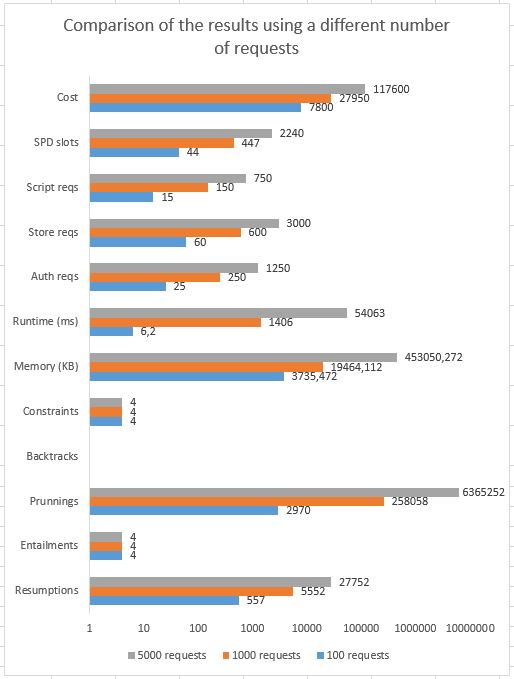
\includegraphics{chart_comp_100_1000_5000.jpg}
\end{center}

No gráfico em cima são comparados as diferentes estatísticas e resultados para três diferentes numéro de pedidos: 100, 1000 e 5000. O número de pedidos de teste é relativamente baixo em relação a um sistema de realidade ou ao que era sugerido no enunciado do problema (cem milhões de pedidos) porque aumentando o número de pedidos aumenta exponencialmente (e de forma bastante acentuada) a RAM e tempo necessário à resolução do problema. Nota-se que para apenas 5000 pedidos, são necessários cerca de 54 segundos e 450 MB de memória RAM.

O número de restrições e vinculações é sempre 4 e o número de retrocessos é sempre 0. O custo, o tempo de execução, memória utilizada, \textit{prunnings} e \textit{resumptions} aumenta exponencialmente com os dados de entrada (de notar que o gráfico apresentado está em escala logarítmica).

\begin{comment}
Demonstrar exemplos de aplicação em casos práticos com  diferentes complexidades e analisar os resultados obtidos. Devem ser utilizadas formas convenientes para apresentação dos resultados (tabelas e/ou gráficos). (Idealmente: comparação de resultados com outros autores/trabalhos.) 
\end{comment}

\section{Conclusões e Perspetivas de Desenvolvimento}\label{sec:Conclusions and Future Work}

A solução que aqui apresentamos é bastante limitada, sem qualquer correspondência a uma situação real. O enunciado do problema original não é realizável em Prolog com recurso aos módulos de PLR, tanto por questões técnicas como também é limitado à quantidade de informação que é capaz de processar, não conseguindo apresentar resultados em tempo de útil quando são usados dados de entrada semelhantes ao que era de esperar num sistema \textit{cloud}.


Não foram feitas referências a outros autores nem trabalhos porque os problemas que são feitos nesta área não correspondem ao problema que aqui apresentamos.

\begin{comment}
Que conclusões retiram deste projeto? O que mostram os resultados obtidos? Quais as vantagens e limitações da solução proposta? (Idealmente: conclusão sobre a comparação com os 
resultados obtidos por outros autores/trabalhos.) Como poderiam melhorar o trabalho desenvolvido?
\end{comment}

\begin{comment}

\begin{thebibliography}{1}

\bibitem{Einstein}
A. Einstein, On the movement of small particles suspended in stationary liquids required by the molecular-kinetic theory of heat, Annalen der Physik 17, pp. 549-560, 1905.

\end{thebibliography}

\end{comment}

\newpage
\appendix
\section{Anexos}

\definecolor{mygreen}{rgb}{0,0.6,0}
\definecolor{mygray}{rgb}{0.5,0.5,0.5}
\definecolor{mymauve}{rgb}{0.58,0,0.82}

\lstset{ %
  backgroundcolor=\color{white},
  basicstyle=\footnotesize,
  breakatwhitespace=false,
  breaklines=true,
  captionpos=b,
  commentstyle=\color{mygreen},
  extendedchars=true,
  keepspaces=true,
  keywordstyle=\color{blue},
  language=Prolog,
  morekeywords={*,...},
  numbers=left,
  numbersep=5pt,
  numberstyle=\tiny\color{mygray},
  rulecolor=\color{black},
  showspaces=false,
  showstringspaces=false,
  showtabs=false,
  stepnumber=1,
  stringstyle=\color{mymauve},
  tabsize=2,
  title=\lstname
}

\subsection{Código Fonte}
\lstinputlisting{tp2.pl}

\subsection{Ficheiro de Configuração}
\lstinputlisting{tp2_config.pl}

\end{document}